\documentclass[10pt]{article}
\usepackage[polish]{babel}
\usepackage[utf8]{inputenc}
\usepackage[T1]{fontenc}
\usepackage{amsmath}
\usepackage{amsfonts}
\usepackage{amssymb}
\usepackage[version=4]{mhchem}
\usepackage{stmaryrd}
\usepackage{graphicx}
\usepackage[export]{adjustbox}
\graphicspath{ {./images/} }
\usepackage{multirow}

\title{MATEMATYKA }

\author{}
\date{}


\newcommand\Varangle{\mathop{{<\!\!\!\!\!\text{\small)}}\:}\nolimits}

\begin{document}
\maketitle
CENTRALNA\\
KOMISJA\\
EGZAMINACYJNA\\
WYPEŁNIA ZDAJĄCY

\begin{center}
\begin{tabular}{l}
KOD \\
\begin{tabular}{|l|l|l|l|l|l|l|l|l|}
\hline
\end{tabular} \\
\hline
\end{tabular}
\end{center}\(\quad\)\begin{tabular}{|l|l|l|l|l|l|}
\hline
 &  &  &  &  &  \\
\hline
\end{tabular}

Arkusz zawiera informacje prawnie chronione do momentu rozpoczęcia egzaminu.

\section*{Miejsce na naklejkę.}
Sprawdż, czy kod na naklejce to E-100.

Jeżeli tak - przyklej naklejkę. Jeżeli nie - zgłoś to nauczycielowi.

Egzamin maturalny

\section*{Poziom rozszerzony}
Symbol arkusza\\
EMAP-RO-100-2305

\section*{DATA: 12 maja 2023 r.}
GoDZINA ROZPOCZECIA: 9:00\\
CZas trWania: \(\mathbf{1 8 0}\) minut

\begin{center}
\begin{tabular}{l}
\(\mid\) WYPEŁNIA ZESPÓŁ NADZORUJACCY \\
\hline
Uprawnienia zdającego do: \\
\(\square\) dostosowania zasad oceniania \\
\(\square\) dostosowania w zw. z dyskalkulią \\
\(\square\) nieprzenoszenia zaznaczeń na kartę. \\
\hline
\end{tabular}
\end{center}

\section*{LICZBA PUNKTÓW DO UZYSKANIA: 50}
\section*{Przed rozpoczęciem pracy z arkuszem egzaminacyjnym}
\begin{enumerate}
  \item Sprawdź, czy nauczyciel przekazał Ci właściwy arkusz egzaminacyjny, tj. arkusz we właściwej formule, z właściwego przedmiotu na właściwym poziomie.
  \item Jeżeli przekazano Ci niewłaściwy arkusz - natychmiast zgłoś to nauczycielowi. Nie rozrywaj banderol.
  \item Jeżeli przekazano Ci właściwy arkusz - rozerwij banderole po otrzymaniu takiego polecenia od nauczyciela. Zapoznaj się z instrukcją na stronie 2.\\

\includegraphics[max width=\textwidth, center]{2024_11_21_c7c9035d1be6a2a9f3d4g-01}
\end{enumerate}

\section*{Instrukcja dla zdającego}
\begin{enumerate}
  \item Sprawdź, czy arkusz egzaminacyjny zawiera 29 stron (zadania 1-16). Ewentualny brak zgłoś przewodniczącemu zespołu nadzorującego egzamin.
  \item Na pierwszej stronie arkusza oraz na karcie odpowiedzi wpisz swój numer PESEL i przyklej naklejkę z kodem.
  \item Odpowiedzi do zadań zamkniętych (1-4) zaznacz na karcie odpowiedzi w części karty przeznaczonej dla zdającego. Zamaluj \(\square\) pola do tego przeznaczone. Błędne zaznaczenie otocz kółkiem i zaznacz właściwe.
  \item W zadaniu 5. wpisz odpowiednie cyfry w kratki pod treścią zadania.
  \item Pamiętaj, że pominięcie argumentacji lub istotnych obliczeń w rozwiązaniu zadania otwartego (6-16) może spowodować, że za to rozwiązanie nie otrzymasz pełnej liczby punktów.
  \item Rozwiązania zadań i odpowiedzi wpisuj w miejscu na to przeznaczonym.
  \item Pisz czytelnie i używaj tylko długopisu lub pióra z czarnym tuszem lub atramentem.
  \item Nie używaj korektora, a błędne zapisy wyraźnie przekreśl.
  \item Nie wpisuj żadnych znaków w części przeznaczonej dla egzaminatora.
  \item Pamiętaj, że zapisy w brudnopisie nie będą oceniane.
  \item Możesz korzystać z Wybranych wzorów matematycznych, cyrkla i linijki oraz kalkulatora prostego. Upewnij się, czy przekazano Ci broszurę z okładką taką jak widoczna poniżej.\\
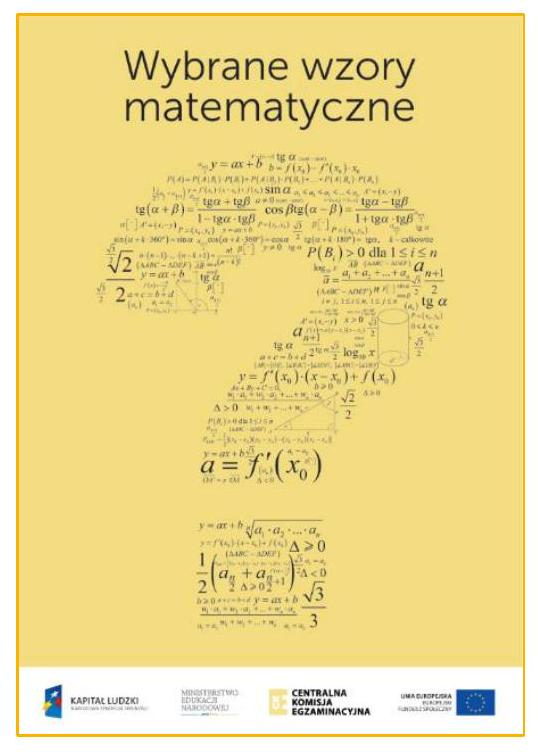
\includegraphics[max width=\textwidth, center]{2024_11_21_c7c9035d1be6a2a9f3d4g-02}
\end{enumerate}

\section*{Zadania egzaminacyjne są wydrukowane na następnych stronach.}
\section*{Zadanie 1. (0-1)}
Granica \(\lim _{x \rightarrow 1} \frac{x^{3}-1}{(x-1)(x+2)}\) jest równa\\
A. \((-1)\)\\
B. 0\\
C. \(\frac{1}{3}\)\\
D. 1

\section*{Zadanie 2. (0-1)}
Dane są wektory \(\vec{u}=[4,-5]\) oraz \(\vec{v}=[-1,-5]\). Długość wektora \(\vec{u}-4 \vec{v}\) jest równa\\
A. 7\\
B. 15\\
C. 17\\
D. 23

\section*{Zadanie 3. (0-1)}
Punkty \(A, B, C, D, E\) leżą na okręgu o środku \(S\). Miara kąta \(B C D\) jest równa \(110^{\circ}\), a miara kąta \(B D A\) jest równa \(35^{\circ}\) (zobacz rysunek).

Wtedy kąt \(D E A\) ma miarę równą\\
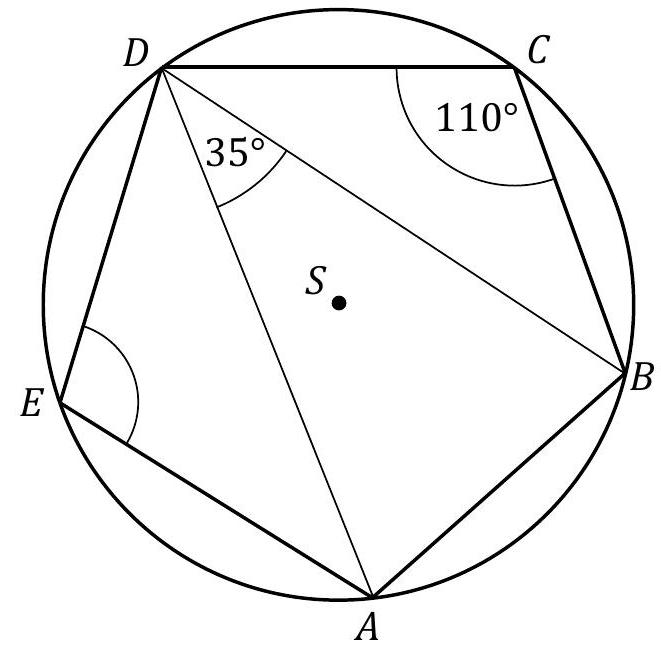
\includegraphics[max width=\textwidth, center]{2024_11_21_c7c9035d1be6a2a9f3d4g-04}\\
A. \(100^{\circ}\)\\
B. \(105^{\circ}\)\\
C. \(110^{\circ}\)\\
D. \(115^{\circ}\)

\section*{Zadanie 4. (0-1)}
Dany jest zbiór trzynastu liczb \(\{1,2,3,4,5,6,7,8,9,10,11,12,13\}\) z z którego losujemy jednocześnie dwie liczby. Wszystkich różnych sposobów wylosowania z tego zbioru dwóch liczb, których iloczyn jest liczbą parzystą, jest\\
A. \(\binom{7}{2}+49\)\\
B. \(\binom{6}{1} \cdot\binom{7}{1}+49\)\\
C. \(\binom{13}{2}-\binom{7}{2}\)\\
D. \(\binom{13}{2}-\binom{6}{2}\)

BRUDNOPIS (nie podlega ocenie)\\

\includegraphics[max width=\textwidth, center]{2024_11_21_c7c9035d1be6a2a9f3d4g-05}

Zadanie 5. (0-2)\\
Wielomian \(W(x)=7 x^{3}-9 x^{2}+9 x-2\) ma dokładnie jeden pierwiastek rzeczywisty. Oblicz ten pierwiastek.

W poniższe kratki wpisz kolejno - od lewej do prawej - pierwszą, drugą oraz trzecią cyfrę po przecinku nieskończonego rozwinięcia dziesiętnego otrzymanego wyniku.\\
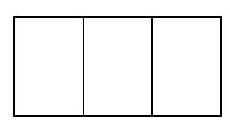
\includegraphics[max width=\textwidth, center]{2024_11_21_c7c9035d1be6a2a9f3d4g-06}

\section*{BRUDNOPIS (nie podlega ocenie)}
\begin{center}

\includegraphics[max width=\textwidth]{2024_11_21_c7c9035d1be6a2a9f3d4g-06(1)}
\end{center}

Zadanie 6. (0-3)\\
Liczby rzeczywiste \(x\) oraz \(y\) spełniają jednocześnie równanie \(x+y=4\) i nierówność \(x^{3}-x^{2} y \leq x y^{2}-y^{3}\). Wykaż, że \(x=2\) oraz \(y=2\).\\

\includegraphics[max width=\textwidth, center]{2024_11_21_c7c9035d1be6a2a9f3d4g-07}

Zadanie 7. (0-3)\\
Dany jest trójkąt prostokątny \(A B C\), w którym \(|\Varangle A B C|=90^{\circ}\) oraz \(|\Varangle C A B|=60^{\circ}\). Punkty \(K\) i \(L\) leżą na bokach - odpowiednio \(-A B\) i \(B C\) tak, że \(|B K|=|B L|=1\) (zobacz rysunek). Odcinek \(K L\) przecina wysokość \(B D\) tego trójkąta w punkcie \(N\), a ponadto \(|A D|=2\).\\
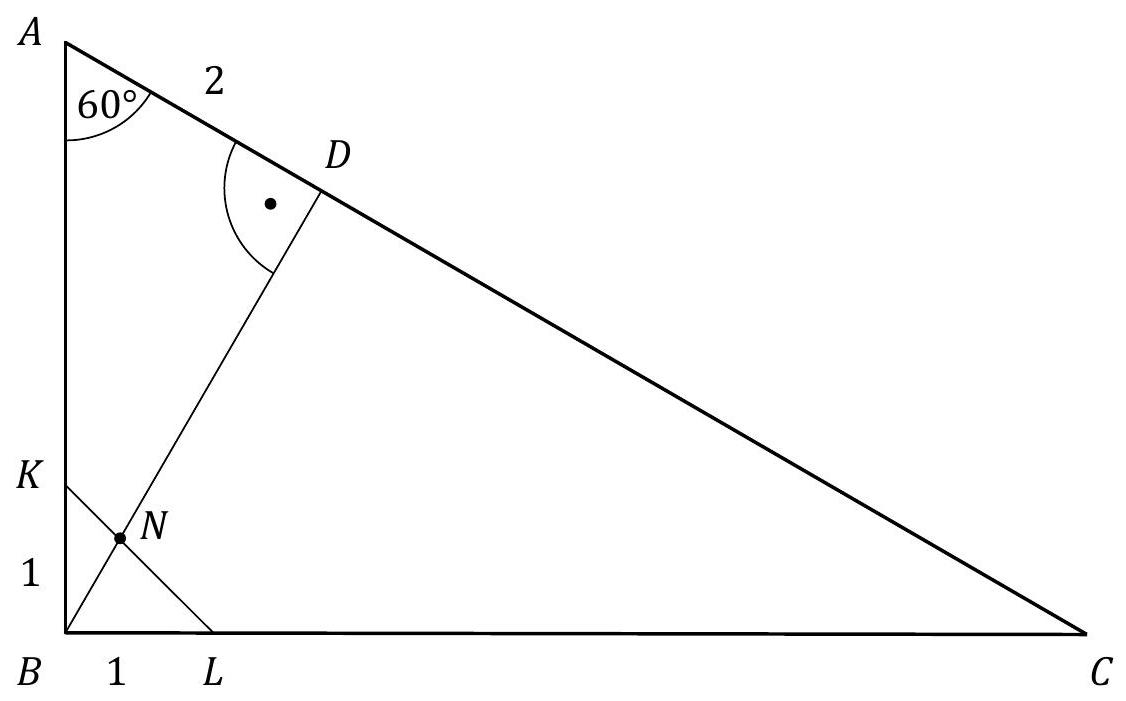
\includegraphics[max width=\textwidth, center]{2024_11_21_c7c9035d1be6a2a9f3d4g-08}

Wykaż, że \(|N D|=\sqrt{3}+1\).\\

\includegraphics[max width=\textwidth, center]{2024_11_21_c7c9035d1be6a2a9f3d4g-08(1)}\\

\includegraphics[max width=\textwidth, center]{2024_11_21_c7c9035d1be6a2a9f3d4g-09}

\begin{center}
\begin{tabular}{|c|l|c|}
\hline
\multirow{3}{*}{\begin{tabular}{c}
Wypełnia \\
egzaminator \\
\end{tabular}} & Nr zadania & 7. \\
\cline { 2 - 3 }
 & Maks. liczba pkt & 3 \\
\cline { 2 - 3 }
 & Uzyskana liczba pkt &  \\
\hline
\end{tabular}
\end{center}

Zadanie 8. (0-3)\\
W pojemniku jest siedem kul: pięć kul białych i dwie kule czarne. Z tego pojemnika losujemy jednocześnie dwie kule bez zwracania. Następnie - z kul pozostałych w pojemniku losujemy jeszcze jedną kulę. Oblicz prawdopodobieństwo wylosowania kuli czarnej w drugim losowaniu.

\begin{center}
\begin{tabular}{|c|c|c|c|c|c|c|c|c|c|c|c|c|c|c|c|c|c|c|c|c|c|c|}
\hline
 &  &  &  &  &  &  &  &  &  &  &  &  &  &  &  &  &  &  &  &  &  &  \\
\hline
 &  &  &  &  &  &  &  &  &  &  &  &  &  &  &  &  &  &  &  &  &  &  \\
\hline
 &  &  &  &  &  &  &  &  &  &  &  &  &  &  &  &  &  &  &  &  &  &  \\
\hline
 &  &  &  &  &  &  &  &  &  &  &  &  &  &  &  &  &  &  &  &  &  &  \\
\hline
 &  &  &  &  &  &  &  &  &  &  &  &  &  &  &  &  &  &  &  &  &  &  \\
\hline
 &  &  &  &  &  &  &  &  &  &  &  &  &  &  &  &  &  &  &  &  &  &  \\
\hline
 &  &  &  &  &  &  &  &  &  &  &  &  &  &  &  &  &  &  &  &  &  &  \\
\hline
 &  &  &  &  &  &  &  &  &  &  &  &  &  &  &  &  &  &  &  &  &  &  \\
\hline
 &  &  &  &  &  &  &  &  &  &  &  &  &  &  &  &  &  &  &  &  &  &  \\
\hline
 &  &  &  &  &  &  &  &  &  &  &  &  &  &  &  &  &  &  &  &  &  &  \\
\hline
 &  &  &  &  &  &  &  &  &  &  &  &  &  &  &  &  &  &  &  &  &  &  \\
\hline
 &  &  &  &  &  &  &  &  &  & - & - & - &  & - &  & - &  &  &  &  &  &  \\
\hline
 &  &  &  &  &  &  &  &  &  &  &  &  &  &  &  &  &  &  &  &  &  &  \\
\hline
 &  &  &  &  &  &  &  &  &  &  &  &  &  &  &  &  &  &  &  &  &  &  \\
\hline
 &  &  &  &  &  &  &  &  &  &  &  &  &  &  &  &  &  &  &  &  &  &  \\
\hline
 &  &  &  &  &  &  &  &  &  &  &  &  &  &  &  &  &  &  &  &  &  &  \\
\hline
 &  &  &  &  &  &  &  &  &  &  &  &  &  &  &  &  &  &  &  &  &  &  \\
\hline
 &  &  &  &  &  &  &  &  &  &  &  &  &  &  &  &  &  &  &  &  &  &  \\
\hline
 &  &  &  &  &  &  &  &  &  &  &  &  &  &  &  &  &  &  &  &  &  &  \\
\hline
 &  &  &  &  &  &  &  &  &  &  &  &  &  &  &  &  &  &  &  &  &  &  \\
\hline
 &  &  &  &  &  &  &  &  &  &  &  &  &  &  &  &  &  &  &  &  &  &  \\
\hline
 &  &  &  &  &  &  &  &  &  &  &  &  &  &  &  &  &  &  &  &  &  &  \\
\hline
 &  &  &  &  &  &  &  &  &  &  &  &  &  &  &  &  &  &  &  &  &  &  \\
\hline
 &  &  &  &  &  &  &  &  &  &  &  &  &  &  &  &  &  &  &  &  &  &  \\
\hline
 &  &  &  &  &  &  &  &  &  &  &  &  &  &  &  &  &  &  &  &  &  &  \\
\hline
 &  &  &  &  &  &  &  &  &  &  &  &  &  &  &  &  &  &  &  &  &  &  \\
\hline
 &  &  &  &  &  &  &  &  &  &  &  &  &  &  &  &  &  &  &  &  &  &  \\
\hline
 &  &  &  &  &  &  &  &  &  &  &  &  &  &  &  &  &  &  &  &  &  &  \\
\hline
 &  &  &  &  &  &  &  &  &  &  &  &  &  &  &  &  &  &  &  &  &  &  \\
\hline
 &  &  &  &  &  &  &  &  &  &  &  &  &  &  &  &  &  &  &  &  &  &  \\
\hline
 &  &  &  &  &  &  &  &  &  &  &  &  &  &  &  &  &  &  &  &  &  &  \\
\hline
 &  &  &  &  &  &  &  &  &  &  &  &  &  &  &  &  &  &  &  &  &  &  \\
\hline
 &  &  &  &  &  &  &  &  &  &  &  &  &  &  &  &  &  &  &  &  &  &  \\
\hline
 &  &  &  &  &  &  &  &  &  &  &  &  &  &  &  &  &  &  &  &  &  &  \\
\hline
 &  &  &  &  &  &  &  &  &  &  &  &  &  &  &  &  &  &  &  &  &  &  \\
\hline
 &  &  &  &  &  &  &  &  &  &  &  &  &  &  &  &  &  &  &  &  &  &  \\
\hline
 &  &  &  &  &  &  &  &  &  &  &  &  &  &  &  &  &  &  &  &  &  &  \\
\hline
 &  &  &  &  &  &  &  &  &  &  &  &  &  &  &  &  &  &  &  &  &  &  \\
\hline
 &  &  &  &  &  &  &  &  &  &  &  &  &  &  &  &  &  &  &  &  &  &  \\
\hline
 &  &  &  &  &  &  &  &  &  &  &  &  &  &  &  &  &  &  &  &  &  &  \\
\hline
 &  &  &  &  &  &  &  &  &  &  &  &  &  &  &  &  &  &  &  &  &  &  \\
\hline
 &  &  &  &  &  &  &  &  &  &  &  &  &  &  &  &  &  &  &  &  &  &  \\
\hline
 &  &  &  &  &  &  &  &  &  &  &  &  &  &  &  &  &  &  &  &  &  &  \\
\hline
\end{tabular}
\end{center}

Zadanie 9. (0-3)\\
Funkcja \(f\) jest określona wzorem \(f(x)=\frac{3 x^{2}-2 x}{x^{2}+2 x+8}\) dla każdej liczby rzeczywistej \(x\). Punkt \(P=\left(x_{0}, 3\right)\) należy do wykresu funkcji \(f\). Oblicz \(x_{0}\) oraz wyznacz równanie stycznej do wykresu funkcji \(f\) w punkcie \(P\).

\begin{center}
\begin{tabular}{|c|l|c|c|}
\hline
\multirow{2}{*}{\begin{tabular}{c}
Wypełnia \\
egzaminator \\
\end{tabular}} & Nr zadania & \(\mathbf{8 .}\) & 9. \\
\cline { 2 - 4 }
 & Maks. liczba pkt & 3 & 3 \\
\cline { 2 - 4 }
 & Uzyskana liczba pkt &  &  \\
\hline
\end{tabular}
\end{center}

Zadanie 10. (0-4)\\
Rozwiąż nierówność

\[
\sqrt{x^{2}+4 x+4}<\frac{25}{3}-\sqrt{x^{2}-6 x+9}
\]

Wskazówka: skorzystaj z tego, że \(\sqrt{a^{2}}=|a|\) dla każdej liczby rzeczywistej \(a\).

\begin{center}
\begin{tabular}{|c|c|c|c|c|c|c|c|c|c|c|c|c|c|c|c|c|c|c|c|c|c|}
\hline
 &  &  &  &  &  &  &  &  &  &  &  &  &  &  &  &  &  &  &  &  &  \\
\hline
 &  &  &  &  &  &  &  &  &  &  &  &  &  &  &  &  &  &  &  &  &  \\
\hline
 &  &  &  &  &  &  &  &  &  &  &  &  &  &  &  &  &  &  &  &  &  \\
\hline
 &  &  &  &  &  &  &  &  &  &  &  &  &  &  &  &  &  &  &  &  &  \\
\hline
 &  &  &  &  &  &  &  &  &  &  &  &  &  &  &  &  &  &  &  &  &  \\
\hline
 &  &  &  &  &  &  &  &  &  &  &  &  &  &  &  &  &  &  &  &  &  \\
\hline
 &  &  &  &  &  &  &  &  &  &  &  &  &  &  &  &  &  &  &  &  &  \\
\hline
 &  &  &  &  &  &  &  &  &  &  &  &  &  &  &  &  &  &  &  &  &  \\
\hline
 &  &  &  &  &  &  &  &  &  &  &  &  &  &  &  &  &  &  &  &  &  \\
\hline
 &  &  &  &  &  &  &  &  &  &  &  &  &  &  &  &  &  &  &  &  &  \\
\hline
 &  &  &  &  &  &  &  &  &  &  &  &  &  &  &  &  &  &  &  &  &  \\
\hline
 &  &  &  &  &  &  &  &  &  &  &  &  &  &  &  &  &  &  &  &  &  \\
\hline
 &  &  &  &  &  &  &  &  &  &  &  &  &  &  &  &  &  &  &  &  &  \\
\hline
 &  &  &  &  &  &  &  &  &  &  &  &  &  &  &  &  &  &  &  &  &  \\
\hline
 &  &  &  &  &  &  &  &  &  &  &  &  &  &  &  &  &  &  &  &  &  \\
\hline
 &  &  &  &  &  &  &  &  &  &  &  &  &  &  &  &  &  &  &  &  &  \\
\hline
 &  &  &  &  &  &  &  &  &  &  &  &  &  &  &  &  &  &  &  &  &  \\
\hline
 &  &  &  &  &  &  &  &  &  &  &  &  &  &  &  &  &  &  &  &  &  \\
\hline
 &  &  &  &  &  &  &  &  &  &  &  &  &  &  &  &  &  &  &  &  &  \\
\hline
 &  &  &  &  &  &  &  &  &  &  &  &  &  &  &  &  &  &  &  &  &  \\
\hline
 &  &  &  &  &  &  &  &  &  &  &  &  &  &  &  &  &  &  &  &  &  \\
\hline
 &  &  &  &  &  &  &  &  &  &  &  &  &  &  &  &  &  &  &  &  &  \\
\hline
 &  &  &  &  &  &  &  &  &  &  &  &  &  &  &  &  &  &  &  &  &  \\
\hline
 &  &  &  &  &  &  &  &  &  &  &  &  &  &  &  &  &  &  &  &  &  \\
\hline
 &  &  &  &  &  &  &  &  &  &  &  &  &  &  &  &  &  &  &  &  &  \\
\hline
 &  &  &  &  &  &  &  &  &  &  &  &  &  &  &  &  &  &  &  &  &  \\
\hline
 &  &  &  &  &  &  &  &  &  &  &  &  &  &  &  &  &  &  &  &  &  \\
\hline
 &  &  &  &  &  &  &  &  &  &  &  &  &  &  &  &  &  &  &  &  &  \\
\hline
 &  &  &  &  &  &  &  &  &  &  &  &  &  &  &  &  &  &  &  &  &  \\
\hline
 &  &  &  &  &  &  &  &  &  &  &  &  &  &  &  &  &  &  &  &  &  \\
\hline
 &  &  &  &  &  &  &  &  &  &  &  &  &  &  &  &  &  &  &  &  &  \\
\hline
 &  &  &  &  &  &  &  &  &  &  &  &  &  &  &  &  &  &  &  &  &  \\
\hline
 &  &  &  &  &  &  &  &  &  &  &  &  &  &  &  &  &  &  &  &  &  \\
\hline
 &  &  &  &  &  &  &  &  &  &  &  &  &  &  &  &  &  &  &  &  &  \\
\hline
 &  &  &  &  &  &  &  &  &  &  &  &  &  &  &  &  &  &  &  &  &  \\
\hline
 &  &  &  &  &  &  &  &  &  &  &  &  &  &  &  &  &  &  &  &  &  \\
\hline
 &  &  &  &  &  &  &  &  &  &  &  &  &  &  &  &  &  &  &  &  &  \\
\hline
 &  &  &  &  &  &  &  &  &  &  &  &  &  &  &  &  &  &  &  &  &  \\
\hline
 &  &  &  &  &  &  &  &  &  &  &  &  &  &  &  &  &  &  &  &  &  \\
\hline
 &  &  &  &  &  &  &  &  &  &  &  &  &  &  &  &  &  &  &  &  &  \\
\hline
 &  &  &  &  &  &  &  &  &  &  &  &  &  &  &  &  &  &  &  &  &  \\
\hline
 &  &  &  &  &  &  &  &  &  &  &  &  &  &  &  &  &  &  &  &  &  \\
\hline
\end{tabular}
\end{center}

\begin{center}

\includegraphics[max width=\textwidth]{2024_11_21_c7c9035d1be6a2a9f3d4g-13}
\end{center}

\begin{center}
\begin{tabular}{|c|l|c|}
\hline
\multirow{2}{*}{\begin{tabular}{c}
Wypełnia \\
egzaminator \\
\end{tabular}} & Nr zadania & 10. \\
\cline { 2 - 3 }
 & Maks. liczba pkt & 4 \\
\cline { 2 - 3 }
 & Uzyskana liczba pkt &  \\
\hline
\end{tabular}
\end{center}

\section*{Zadanie 11. (0-4)}
Określamy kwadraty \(K_{1}, K_{2}, K_{3}, \ldots\) następująco:

\begin{itemize}
  \item \(K_{1}\) jest kwadratem o boku długości \(a\)
  \item \(K_{2}\) jest kwadratem, którego każdy wierzchołek leży na innym boku kwadratu \(K_{1}\) i dzieli ten bok w stosunku 1:3
  \item \(K_{3}\) jest kwadratem, którego każdy wierzchołek leży na innym boku kwadratu \(K_{2}\) i dzieli ten bok w stosunku 1:3\\
i ogólnie, dla każdej liczby naturalnej \(n \geq 2\),
  \item \(K_{n}\) jest kwadratem, którego każdy wierzchołek leży na innym boku kwadratu \(K_{n-1}\) i dzieli ten bok w stosunku 1:3.\\
Obwody wszystkich kwadratów określonych powyżej tworzą nieskończony ciąg geometryczny.\\
Na rysunku przedstawiono kwadraty utworzone w sposób opisany powyżej.\\
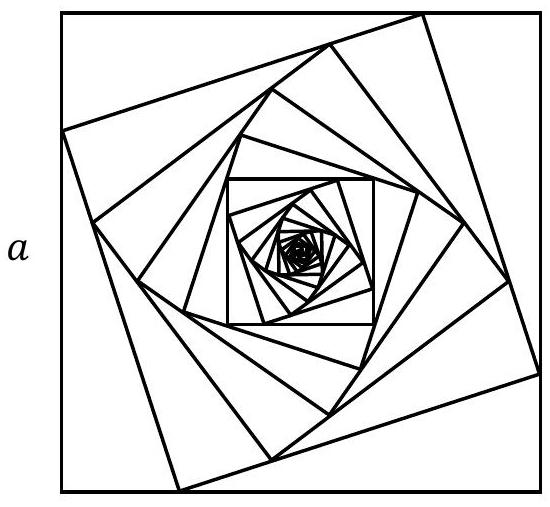
\includegraphics[max width=\textwidth, center]{2024_11_21_c7c9035d1be6a2a9f3d4g-14}\\
a\\
Oblicz sumę wszystkich wyrazów tego nieskończonego ciągu.\\

\includegraphics[max width=\textwidth, center]{2024_11_21_c7c9035d1be6a2a9f3d4g-14(1)}\\

\includegraphics[max width=\textwidth, center]{2024_11_21_c7c9035d1be6a2a9f3d4g-15}
\end{itemize}

\begin{center}
\begin{tabular}{|c|l|c|}
\hline
\multirow{2}{*}{\begin{tabular}{c}
Wypełnia \\
egzaminator \\
\end{tabular}} & Nr zadania & 11. \\
\cline { 2 - 3 }
 & Maks. liczba pkt & 4 \\
\cline { 2 - 3 }
 & Uzyskana liczba pkt &  \\
\hline
\end{tabular}
\end{center}

Zadanie 12. (0-4)\\
Rozwiąż równanie \(3 \sin ^{2} x-\sin ^{2}(2 x)=0 \mathrm{w}\) przedziale \(\langle\pi, 2 \pi\rangle\).\\

\includegraphics[max width=\textwidth, center]{2024_11_21_c7c9035d1be6a2a9f3d4g-16}\\

\includegraphics[max width=\textwidth, center]{2024_11_21_c7c9035d1be6a2a9f3d4g-17}

\begin{center}
\begin{tabular}{|c|l|c|}
\hline
\multirow{2}{*}{\begin{tabular}{c}
Wypełnia \\
egzaminator \\
\end{tabular}} & Nr zadania & 12. \\
\cline { 2 - 3 }
 & Maks. liczba pkt & 4 \\
\cline { 2 - 3 }
 & Uzyskana liczba pkt &  \\
\hline
\end{tabular}
\end{center}

Zadanie 13. (0-4)\\
Czworokąt \(A B C D\), w którym \(|B C|=4\) i \(|C D|=5\), jest opisany na okręgu. Przekątna \(A C\) tego czworokąta tworzy z bokiem \(B C\) kąt o mierze \(60^{\circ}\), natomiast z bokiem \(A B\)-kąt ostry, którego sinus jest równy \(\frac{1}{4}\). Oblicz obwód czworokąta \(A B C D\).

\begin{center}
\begin{tabular}{|c|c|c|c|c|c|c|c|c|c|c|c|c|c|c|c|c|c|c|c|c|c|}
\hline
 &  &  &  &  &  &  &  &  &  &  &  &  &  &  &  &  &  &  &  &  &  \\
\hline
 &  &  &  &  &  &  &  &  &  &  &  &  &  &  &  &  &  &  &  &  &  \\
\hline
 &  &  &  &  &  &  &  &  &  &  &  &  &  &  &  &  &  &  &  &  &  \\
\hline
 &  &  &  &  &  &  &  &  &  &  &  &  &  &  &  &  &  &  &  &  &  \\
\hline
 &  &  &  &  &  &  &  &  &  &  &  &  &  &  &  &  &  &  &  &  &  \\
\hline
 &  &  &  &  &  &  &  &  &  &  &  &  &  &  &  &  &  &  &  &  &  \\
\hline
 &  &  &  &  &  &  &  &  &  &  &  &  &  &  &  &  &  &  &  &  &  \\
\hline
 &  &  &  &  &  &  &  &  &  &  &  &  &  &  &  &  &  &  &  &  &  \\
\hline
 &  &  &  &  &  &  &  &  &  &  &  &  &  &  &  &  &  &  &  &  &  \\
\hline
 &  &  &  &  &  &  &  &  &  &  &  &  &  &  &  &  &  &  &  &  &  \\
\hline
 &  &  &  &  &  &  &  &  &  &  &  &  &  &  &  &  &  &  &  &  &  \\
\hline
 &  &  &  &  &  &  &  &  &  &  &  &  &  &  &  &  &  &  &  &  &  \\
\hline
 &  &  &  &  &  &  &  &  &  &  &  &  &  &  &  &  &  &  &  &  &  \\
\hline
 &  &  &  &  &  &  &  &  &  &  &  &  &  &  &  &  &  &  &  &  &  \\
\hline
 &  &  &  &  &  &  &  &  &  &  &  &  &  &  &  &  &  &  &  &  &  \\
\hline
 &  &  &  &  &  &  &  &  &  &  &  &  &  &  &  &  &  &  &  &  &  \\
\hline
 &  &  &  &  &  &  &  &  &  &  &  &  &  &  &  &  &  &  &  &  &  \\
\hline
 &  &  &  &  &  &  &  &  &  &  &  &  &  &  &  &  &  &  &  &  &  \\
\hline
 &  &  &  &  &  &  &  &  &  &  &  &  &  &  &  &  &  &  &  &  &  \\
\hline
 &  &  &  &  &  &  &  &  &  &  &  &  &  &  &  &  &  &  &  &  &  \\
\hline
 &  &  &  &  &  &  &  &  &  &  &  &  &  &  &  &  &  &  &  &  &  \\
\hline
 &  &  &  &  &  &  &  &  &  &  &  &  &  &  &  &  &  &  &  &  &  \\
\hline
 &  &  &  &  &  &  &  &  &  &  &  &  &  &  &  &  &  &  &  &  &  \\
\hline
 &  &  &  &  &  &  &  &  &  &  &  &  &  &  &  &  &  &  &  &  &  \\
\hline
 &  &  &  &  &  &  &  &  &  &  &  &  &  &  &  &  &  &  &  &  &  \\
\hline
 &  &  &  &  &  &  &  &  &  &  &  &  &  &  &  &  &  &  &  &  &  \\
\hline
 &  &  &  &  &  &  &  &  &  &  &  &  &  &  &  &  &  &  &  &  &  \\
\hline
 &  &  &  &  &  &  &  &  &  &  &  &  &  &  &  &  &  &  &  &  &  \\
\hline
 &  &  &  &  &  &  &  &  &  &  &  &  &  &  &  &  &  &  &  &  &  \\
\hline
 &  &  &  &  &  &  &  &  &  &  &  &  &  &  &  &  &  &  &  &  &  \\
\hline
 &  &  &  &  &  &  &  &  &  &  &  &  &  &  &  &  &  &  &  &  &  \\
\hline
 &  &  &  &  &  &  &  &  &  &  &  &  &  &  &  &  &  &  &  &  &  \\
\hline
 &  &  &  &  &  &  &  &  &  &  &  &  &  &  &  &  &  &  &  &  &  \\
\hline
 &  &  &  &  &  &  &  &  &  &  &  &  &  &  &  &  &  &  &  &  &  \\
\hline
 &  &  &  &  &  &  &  &  &  &  &  &  &  &  &  &  &  &  &  &  &  \\
\hline
 &  &  &  &  &  &  &  &  &  &  &  &  &  &  &  &  &  &  &  &  &  \\
\hline
 &  &  &  &  &  &  &  &  &  &  &  &  &  &  &  &  &  &  &  &  &  \\
\hline
 &  &  &  &  &  &  &  &  &  &  &  &  &  &  &  &  &  &  &  &  &  \\
\hline
 &  &  &  &  &  &  &  &  &  &  &  &  &  &  &  &  &  &  &  &  &  \\
\hline
 &  &  &  &  &  &  &  &  &  &  &  &  &  &  &  &  &  &  &  &  &  \\
\hline
 &  &  &  &  &  &  &  &  &  &  &  &  &  &  &  &  &  &  &  &  &  \\
\hline
 &  &  &  &  &  &  &  &  &  &  &  &  &  &  &  &  &  &  &  &  &  \\
\hline
 &  &  &  &  &  &  &  &  &  &  &  &  &  &  &  &  &  &  &  &  &  \\
\hline
\end{tabular}
\end{center}

\begin{center}

\includegraphics[max width=\textwidth]{2024_11_21_c7c9035d1be6a2a9f3d4g-19}
\end{center}

\begin{center}
\begin{tabular}{|c|l|c|}
\hline
\multirow{2}{*}{\begin{tabular}{c}
Wypełnia \\
egzaminator \\
\end{tabular}} & Nr zadania & 13. \\
\cline { 2 - 3 }
 & Maks. liczba pkt & 4 \\
\cline { 2 - 3 }
 & Uzyskana liczba pkt &  \\
\hline
\end{tabular}
\end{center}

Zadanie 14. (0-4)\\
Dany jest sześcian ABCDEFGH o krawędzi długości 6. Punkt \(S\) jest punktem przecięcia przekątnych \(A H\) i \(D E\) ściany bocznej \(A D H E\) (zobacz rysunek).\\
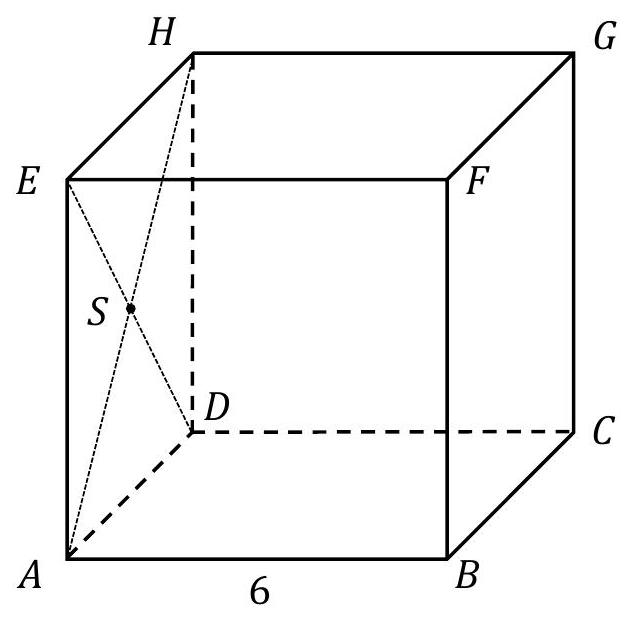
\includegraphics[max width=\textwidth, center]{2024_11_21_c7c9035d1be6a2a9f3d4g-20}

Oblicz wysokość trójkąta SBH poprowadzoną z punktu \(S\) na bok BH tego trójkąta.\\

\includegraphics[max width=\textwidth, center]{2024_11_21_c7c9035d1be6a2a9f3d4g-20(1)}\\

\includegraphics[max width=\textwidth, center]{2024_11_21_c7c9035d1be6a2a9f3d4g-21}

\begin{center}
\begin{tabular}{|c|l|c|}
\hline
\multirow{3}{*}{\begin{tabular}{c}
Wypełnia \\
egzaminator \\
\end{tabular}} & Nr zadania & 14. \\
\cline { 2 - 3 }
 & Maks. liczba pkt & 4 \\
\cline { 2 - 3 }
 & Uzyskana liczba pkt &  \\
\hline
\end{tabular}
\end{center}

Zadanie 15. (0-5)\\
Wyznacz wszystkie wartości parametru \(m \neq 2\), dla których równanie

\[
x^{2}+4 x-\frac{m-3}{m-2}=0
\]

ma dwa różne rozwiązania rzeczywiste \(x_{1}, x_{2}\) spełniające warunek \(x_{1}^{3}+x_{2}^{3}>-28\).

\begin{center}
\begin{tabular}{|c|c|c|c|c|c|c|c|c|c|c|c|c|c|c|c|c|c|c|c|c|c|c|}
\hline
 &  &  &  &  &  &  &  &  &  &  &  &  &  &  &  &  &  &  &  &  &  &  \\
\hline
 &  &  &  &  &  &  &  &  &  &  &  &  &  &  &  &  &  &  &  &  &  &  \\
\hline
 &  &  &  &  &  &  &  &  &  &  &  &  &  &  &  &  &  &  &  &  &  &  \\
\hline
 &  &  &  &  &  &  &  &  &  &  &  &  &  &  &  &  &  &  &  &  &  &  \\
\hline
 &  &  &  &  &  &  &  &  &  &  &  &  &  &  &  &  &  &  &  &  &  &  \\
\hline
 &  &  &  &  &  &  &  &  &  &  &  &  &  &  &  &  &  &  &  &  &  &  \\
\hline
 &  &  &  &  &  &  &  &  &  &  &  &  &  &  &  &  &  &  &  &  &  &  \\
\hline
 &  &  &  &  &  &  &  &  &  &  &  &  &  &  &  &  &  &  &  &  &  &  \\
\hline
 &  &  &  &  &  &  &  &  &  &  &  &  &  &  &  &  &  &  &  &  &  &  \\
\hline
 &  &  &  &  &  &  &  &  &  &  &  &  &  &  &  &  &  &  &  &  &  &  \\
\hline
 &  &  &  &  &  &  &  &  &  &  &  &  &  &  &  &  &  &  &  &  &  &  \\
\hline
 &  &  &  &  &  &  &  &  &  &  &  &  &  &  &  &  &  &  &  &  &  &  \\
\hline
 &  &  &  &  &  &  &  &  &  &  &  &  &  &  &  &  &  &  &  &  &  &  \\
\hline
 &  &  &  &  &  &  &  &  &  &  &  &  &  &  &  &  &  &  &  &  &  &  \\
\hline
 &  &  &  &  &  &  &  &  &  &  &  &  &  &  &  &  &  &  &  &  &  &  \\
\hline
 &  &  &  &  &  &  &  &  &  &  &  &  &  &  &  &  &  &  &  &  &  &  \\
\hline
 &  &  &  &  &  &  &  &  &  &  &  &  &  &  &  &  &  &  &  &  &  &  \\
\hline
 &  &  &  &  &  &  &  &  &  &  &  &  &  &  &  &  &  &  &  &  &  &  \\
\hline
 &  &  &  &  &  &  &  &  &  &  &  &  &  &  &  &  &  &  &  &  &  &  \\
\hline
 &  &  &  &  &  &  &  &  &  &  &  &  &  &  &  &  &  &  &  &  &  &  \\
\hline
 &  &  &  &  &  &  &  &  &  &  &  &  &  &  &  &  &  &  &  &  &  &  \\
\hline
 &  &  &  &  &  &  &  &  &  &  &  &  &  &  &  &  &  &  &  &  &  &  \\
\hline
 &  &  &  &  &  &  &  &  &  &  &  &  &  &  &  &  &  &  &  &  &  &  \\
\hline
 &  &  &  &  &  &  &  &  &  &  &  &  &  &  &  &  &  &  &  &  &  &  \\
\hline
 &  &  &  &  &  &  &  &  &  &  &  &  &  &  &  &  &  &  &  &  &  &  \\
\hline
 &  &  &  &  &  &  &  &  &  &  &  &  &  &  &  &  &  &  &  &  &  &  \\
\hline
 &  &  &  &  &  &  &  &  &  &  &  &  &  &  &  &  &  &  &  &  &  &  \\
\hline
 &  &  &  &  &  &  &  &  &  &  &  &  &  &  &  &  &  &  &  &  &  &  \\
\hline
 &  &  &  &  &  &  &  &  &  &  &  &  &  &  &  &  &  &  &  &  &  &  \\
\hline
 &  &  &  &  &  &  &  &  &  &  &  &  &  &  &  &  &  &  &  &  &  &  \\
\hline
 &  &  &  &  &  &  &  &  &  &  &  &  &  &  &  &  &  &  &  &  &  &  \\
\hline
 &  &  &  &  &  &  &  &  &  &  &  &  &  &  &  &  &  &  &  &  &  &  \\
\hline
 &  &  &  &  &  &  &  &  &  &  &  &  &  &  &  &  &  &  &  &  &  &  \\
\hline
 &  &  &  &  &  &  &  &  &  &  &  &  &  &  &  &  &  &  &  &  &  &  \\
\hline
 &  &  &  &  &  &  &  &  &  &  &  &  &  &  &  &  &  &  &  &  &  &  \\
\hline
 &  &  &  &  &  &  &  &  &  &  &  &  &  &  &  &  &  &  &  &  &  &  \\
\hline
 &  &  &  &  &  &  &  &  &  &  &  &  &  &  &  &  &  &  &  &  &  &  \\
\hline
 &  &  &  &  &  &  &  &  &  &  &  &  &  &  &  &  &  &  &  &  &  &  \\
\hline
 &  &  &  &  &  &  &  &  &  &  &  &  &  &  &  &  &  &  &  &  &  &  \\
\hline
 &  &  &  &  &  &  &  &  &  &  &  &  &  &  &  &  &  &  &  &  &  &  \\
\hline
 &  &  &  &  &  &  &  &  &  &  &  &  &  &  &  &  &  &  &  &  &  &  \\
\hline
\end{tabular}
\end{center}

\begin{center}

\includegraphics[max width=\textwidth]{2024_11_21_c7c9035d1be6a2a9f3d4g-23}
\end{center}

\begin{center}
\begin{tabular}{|c|l|c|}
\hline
\multirow{2}{*}{\begin{tabular}{c}
Wypełnia \\
egzaminator \\
\end{tabular}} & Nr zadania & 15. \\
\cline { 2 - 3 }
 & Maks. liczba pkt & 5 \\
\cline { 2 - 3 }
 & Uzyskana liczba pkt &  \\
\hline
\end{tabular}
\end{center}

Zadanie 16. (0-7)\\
Rozważamy trójkąty \(A B C\), w których \(A=(0,0), B=(m, 0)\), gdzie \(m \in(4,+\infty)\), a wierzchołek \(C\) leży na prostej o równaniu \(y=-2 x\). Na boku \(B C\) tego trójkąta leży punkt \(D=(3,2)\).\\
a) Wykaż, że dla \(m \in(4,+\infty)\) pole \(P\) trójkąta \(A B C\), jako funkcja zmiennej \(m\), wyraża się wzorem

\[
P(m)=\frac{m^{2}}{m-4}
\]

b) Oblicz tę wartość \(m\), dla której funkcja \(P\) osiąga wartość najmniejszą. Wyznacz równanie prostej \(B C\), przy której funkcja \(P\) osiąga tę najmniejszą wartość.\\

\includegraphics[max width=\textwidth, center]{2024_11_21_c7c9035d1be6a2a9f3d4g-24}\\

\includegraphics[max width=\textwidth, center]{2024_11_21_c7c9035d1be6a2a9f3d4g-25}\\

\includegraphics[max width=\textwidth, center]{2024_11_21_c7c9035d1be6a2a9f3d4g-26}

\begin{center}
\begin{tabular}{|c|l|c|}
\hline
\multirow{3}{*}{\begin{tabular}{c}
Wypełnia \\
egzaminator \\
\end{tabular}} & Nr zadania & 16. \\
\cline { 2 - 3 }
 & Maks. liczba pkt & 7 \\
\cline { 2 - 3 }
 & Uzyskana liczba pkt &  \\
\hline
\end{tabular}
\end{center}

BRUDNOPIS (nie podlega ocenie)\\

\includegraphics[max width=\textwidth, center]{2024_11_21_c7c9035d1be6a2a9f3d4g-27}\\

\includegraphics[max width=\textwidth, center]{2024_11_21_c7c9035d1be6a2a9f3d4g-28}\\

\includegraphics[max width=\textwidth, center]{2024_11_21_c7c9035d1be6a2a9f3d4g-29}

\section*{MATEMATYKA}
\section*{Poziom rozszerzony}
Formuła 2015

\section*{MATEMATYKA}
Poziom rozszerzony Formuła 2015

\section*{MATEMATYKA}
Poziom rozszerzony\\
Formuła 2015


\end{document}